\chapter{The RoFI Prototypes}\label{chap:prototypes}

The RoFI project as defined in the previous chapter is broad and, therefore,
implementing all of the proposed solutions in the full depth is far beyond the
reach of the thesis. Therefore, we focused on three of the most important
aspects of the RoFI project. We want to show that:
\begin{itemize}
    \item the docking mechanism can be built and that it features claimed
    properties,
    \item integration of TCP/IP communication in the system using a custom
    hardware layer is possible, and
    \item the universal module can be built.
\end{itemize}

All the source codes and CAD models of results presented here are available at
\url{https://github.com/paradise-fi/RoFi}.

\section{Docking Mechanism}

To test the properties of the docking mechanism proposed in section
\ref{sec:dock} we successfully built several copies of the mechanism and tested
its properties.

The docks can be easily printed on a commonly available 3D printer. In our
setting, the dock was printed on Prusa i3 MK3 using the PLA filament and
standard settings with a layer height of 0.15~mm. We prepared the model for
printing by splitting some complex components into several bodies, which
were printed separately, and after the print they were glued together using
cyanoacrylate glue. As our experiences show, such procedure yields better and
faster results as our model does not need any support material, which needs to
been manually removed. Removing the support material is time-consuming and in
our observation, gluing components together is much faster. Also, surfaces
relying on a support material always yields much worse surface finish than
surfaces with no supports. This is crucial for our model, as a bad surface
finish on the helix slot negatively affects the dock.

Overall, to build a single dock following material is needed: eight meters of a
filament, four M2$\times$6~mm screws with countersunk head, two 2$\times$16~mm
steel pins, four 2$\times$10~mm, four 2$\times$8~mm stell pins and a motor.
Single dock takes about 4 hours to print and with a little bit of practice, it
can be assembled in 30 minutes. Due to tweaks in the design, there is
practically no manual deburring necessary, which is usually required with 3D
printed parts.

We tried to evaluate the features of the dock. However, please note that the
results we present are not as thorough as could be as we do not feature the
equipment and skills to evaluate the mechanical properties of the docks
properly.

\begin{figure}[!t]
    \centering
    \includegraphics[width=\textwidth]{figures/dock_test_setup.jpg}
    \caption{The test setup. A stand was mounted on the docks to easily position
    them and a printed grid was used to create various setups.}
    \label{fig:dock_test_setup}
\end{figure}

\begin{figure}[!t]
    \centering
    \begin{subfigure}[b]{0.45\textwidth}
        \includegraphics[width=\textwidth]{figures/docks_aligned.jpg}
        \caption{Perfect alignment}
        \label{fig:dock_test_aligned}
    \end{subfigure}
    ~
    \begin{subfigure}[b]{0.45\textwidth}
        \includegraphics[width=\textwidth]{figures/docks_distance.jpg}
        \caption{Distance misplacement}
        \label{fig:dock_test_distance}
    \end{subfigure}

    \begin{subfigure}[b]{0.45\textwidth}
        \includegraphics[width=\textwidth]{figures/docks_shift.jpg}
        \caption{Parallel misplacement}
        \label{fig:dock_test_parallel}
    \end{subfigure}
    ~
    \begin{subfigure}[b]{0.45\textwidth}
        \includegraphics[width=\textwidth]{figures/docks_rot.jpg}
        \caption{Rotational alignment}
        \label{fig:dock_test_rot}
    \end{subfigure}

    \caption{Types of displacement.}
    \label{fig:dock_diplacement}
\end{figure}

To properly evaluate the docks, we 3D printed a stand on which a single dock was
mounted. The docks we used for testing were manually controlled. A photo of our
setup can be found in figure \ref{fig:dock_test_setup}. This setup was used for
testing of connection repeatability and load capacity.

\subsection{Connection repeatability}

Two docking mechanisms were brought together in various arrangements and a
series of 10 connects was performed. The docks were placed on a grid to arrange
them in the initial position with one dock being strongly fixed in its position,
the other one being able to move.

First, we performed an analysis of perfectly aligned docks (see figure
\ref{fig:dock_test_aligned}). The connection was established in all 10 cases for
both, simultaneous and sequential docking procedure.

Second, we varied the docking distance (see figure
\ref{fig:dock_test_distance}). By decreasing the docking distance by 6~mm, the
docks were able to push themselves apart and connect properly in all 10 cases.
When the docks were brought together by more than 6~mm, we observed that the
docks are not able to connect simultaneously -- their hooks collide and they do
not align properly. However, when the connection was performed sequentially, the
docks connected reliably event when they were touching as the rotated hooks no
longer collide. By increasing the distance by 2~mm, docks were able to connect
in 9 out of 10 cases. When we increased the distance by 4~mm docks were able to
connect in 5 cases. For displacement larger than 5~mm the docs were not able to
connect.

Third, we varied the parallel alignment (see figure
\ref{fig:dock_test_parallel}). By misaligning the docks by 2~mm we got 9
successfully connections. By increasing the misalignment to 4~mm the docks
connected in 6 cases, for the 6~mm it was only 3 cases. We did not observed ony
difference between simultaneous and sequential attempts.

Last, we varied the rotation of the docks (see figure \ref{fig:dock_test_rot}).
We performed an only rotation in a horizontal plane as the docs are symmetric
and therefore, they should perform the same for other orientations. By rotating
the docks less than $5^\circ$ the docks connected in all 10 cases. When we
increased the rotation to $10^\circ$, we got 7 successful connections for
sequential connection and 5 for the simultaneous connection. For displacement of
$15^\circ$ we got only 1 connection of 10 tries for the sequential connection
and no success for the simultaneous procedure.

When the connection was not successful it was mainly due to the hooks colliding
into each other. The collision usually caused a motor stall, which can be easily
detected by increasing current flow into the motor. This fact could be used by the
robots to detect such collision, and the robots could retry the connection.

\subsection{Load capacity}

\begin{figure}[t!]
    \centering
    \begin{subfigure}[b]{0.45\textwidth}
        \includegraphics[width=\textwidth]{figures/dock_tang_load.jpg}
        \caption{Tangential stress}
        \label{fig:dock_test_tang}
    \end{subfigure}
    ~
    \begin{subfigure}[b]{0.45\textwidth}
        \includegraphics[width=\textwidth]{figures/dock_norm_load.jpg}
        \caption{Normal stress}
        \label{fig:dock_test_norm}
    \end{subfigure}
    \caption{Testing load capacity of the docks. The load was attached to the
    green carabiner.}
    \label{fig:dock_test_load}
\end{figure}

We tested load capacity in two different setups -- in a tangential and a normal
direction (see figure \ref{fig:dock_test_load}) -- by attaching weights to a
carabiner hooked to one of the connected docks. The mating dock was fixed to a
support.

In a normal direction, we were able to repeatably attach a weight of 4.5~kg
until the docks disconnected. The disconnection left no harm on the docks. We
assume the plastic hooks bent under the load as the plastic is quite flexible,
the skirts got loose and therefore, the the docks were able to slip from the
connection.

\begin{figure}[t!]
    \centering
    \begin{subfigure}[b]{0.45\textwidth}
        \includegraphics[width=\textwidth]{figures/dock_damage_1.jpg}
        \caption{Dock hooks}
    \end{subfigure}
    ~
    \begin{subfigure}[b]{0.45\textwidth}
        \includegraphics[width=\textwidth]{figures/dock_damage_2.jpg}
        \caption{Pieces of the hooks broken apart}
    \end{subfigure}
    \caption{Damage caused by load testing on the docks.}
    \label{fig:dock_damage}
\end{figure}

In a tangential direction, we were able to attach weight of 8~kg until the
malfunction of connection happened. In this case, the connection mechanism was
damaged -- two hooks on one dock and one hook on the other dock broke. For a
photo of the damage see figure \ref{fig:dock_damage}. The pieces were broken
between two layers of the 3D printed component. The form of the damage leads us
to a suggestion for future experiments -- printing the hooks such that the
layers of a 3D print are oriented differently.


\section{Inter-module Communication}

We proposed in section \ref{sec:communication} that the modules in a RoFI system
should communicate using a TCP/IP networking as it allows to easily adapt
existing algorithms and technical solutions. The proposed solution implements a
custom layer two of the standard ISO/OSI model.

To show the feasibility of the proposed solution, we have implemented a simple
prototype. The prototype does not provide any mechanical hardware, it consists
only of several interconnected development modules with microcontrollers. We
implemented a firmware for the ATMega328p microcontroller providing the dock
protocol (section \ref{sec:dock_interface}) and a corresponding part of the RoFI
driver for the ESP32 microcontroller -- dock driver, address mapping protocol
and interface for the lwIP TCP/IP stack. Both implementations can be found in the
project repository.

The ATMega328p was chosen due availability of cheap development modules in form
Arduino Nano and low-effort development. This decision allowed us to quickly get
a working prototype, however, at the cost of not providing a solution with high
performance as we reached memory and computational limits of the
microcontroller. The limitations come in form of limited SPI clock speed
(100~kHz) and smaller maximal blob size (128 bytes). We consider the
implementation of the firmware straightforward and not worth further
description.

On the other hand, the implementation of the RoFI driver for ESP32 we provide is
intended for future use. The driver is written in C++14. It is structured in two
classes: \texttt{Dock} (direct interface for a single dock) and \texttt{Roif}
(network interface built on top docks).

\texttt{Dock} automatically handles communication with the docks, i.e., hides
all details of the communication (e.g., interrupt handling) and provides a
simple interface: user can supply a binary blob (in form of the \texttt{pbuf}
structure from lwIP) or be notified with an incoming blob via a callback. The
interface for changing or querying dock state (retracting or expanding of the
dock, querying the state of the power lines, etc.) is implemented in a similar
fashion. Our implementation prevents congestion of the shared SPI bus by
limiting the number of pending queries per dock and therefore, allowing for fair
usage of the bus.

The challenge of the implementation was mapping SPI transaction to the interface
provided by ESP32 development framework (ESP-IDF). ESP-IDF provides a way to
queue asynchronous SPI transactions with distinct read and write phases
including delay between the phases. However, it does not support transactions
with variable length, which are required by our protocol. The transactions have
to be implemented using several SPI transaction offered by ESP-IDF. The naive
implementation is not possible as transactions from multiple docks could
interleave and therefore, yield incorrect results. There are two possible
approaches to tackle this problem: we can either queue transactions in advance
and modify them on the fly, or we can use a separate FreeRTOS task executing
blocking SPI transactions. Our implementation uses the second solution as our
analysis of the ESP-IDF source code shows that changing already queued
transactions is not safe and also, the first solution requires non-trivial
locking. The second solution also produces easier to follow code with no
explicit locking as all the locking is handled by FreeRTOS and therefore, was
chosen.

\texttt{Roif} (\emph{Ro}Fi network \emph{in}terface) provides a glue between
docks and lwIP. It handles registration of a new network interface and all the
required callbacks (as we mentioned in section \ref{sec:networking}). It also
features implementation of the address mapping protocol to determine which dock
should be used for outgoing communication.

As a by-product of the implementation of the RoFI driver, we implemented a set
of C++ wrappers for the FreeRTOS API. Unlike the already existing C++ wrappers
we are aware of, we do not simply rename functions and group them in classes
like these wrappers. Our wrappers respect C++ idioms and also provide proper C++
copy and move semantics. Such wrapper allows the user to write easier to
understand and less error-prone code. At the time of writing this thesis, the
FreeRTOS wrapper was not separated into a stand-alone project.

\begin{figure}[!t]
    \centering
    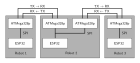
\includegraphics[width=\textwidth]{figures/communication_setup.pdf}
    \caption{The setup for our inter-module communication prototype. Physical
    realization is shown in figure \ref{fig:comm_setup_p}.}
    \label{fig:comm_setup}
\end{figure}

\begin{figure}[!t]
    \centering
    \includegraphics[width=\textwidth]{figures/com_setup.jpg}
    \caption{Physical realization of the setup shown in figure \ref{fig:comm_setup}.}
    \label{fig:comm_setup_p}
\end{figure}

We tested our implementation in a simple setup shown at figure
\ref{fig:comm_setup}. We used three ESP32-DevkitCs simulating module
controllers, and for Arduino Nanos simulating the docks. We wired them as shown
in the figure. Then, we were able to successfully establish both, TCP and UDP,
connections. The codes for establishing the connections are a simple example
inspired by official demo codes. There are no modifications for our setup. The
example codes can be found in the project repository.

Replication of our results should be fairly straightforward as we ship all the
code as PlatformIO\footnote{\url{https://platformio.org/}} projects, therefore
no complicated toolchain setup is necessary; and also, the hardware we use is
commonly available. However, during testing of our firmware, we encountered a
bug in lwIP implementation preventing a TCP connection from being opened. The
bug has been already fixed in the lwIP upstream repository, however, at the time
of writing this thesis, the lwIP library shipped with ESP-IDF was not updated.
Therefore, to successfully run the TCP example, manual update of the library is
necessary.

\section{Universal Module}

So far, we have built several prototypes of the universal module; some of the
key iterations are shown in figure \ref{fig:um_evolution}. There were several
challenges during the design of the module; first, the module should be as rigid
as possible to be able to support large structures of RoFI systems (this is
challenging mainly due to the presence of the $\gamma$-axis), second, the
internal arrangement of components have to be compact to fit in the 10cm cube
grid and third, the module should be strong to lift at least two other robots.

\begin{figure}[!t]
    \centering
    \includegraphics[width=\textwidth]{figures/um_evolution.jpg}
    \caption{Evolution of the universal module. First paper prototype (left),
    first 3D printed version (middle), and the current state (right).}
    \label{fig:um_evolution}
\end{figure}

The last prototype (figures \ref{fig:um_photo_side} and \ref{fig:um_photo_top})
fulfills our goals -- it features rigid construction and we were able to fit
sufficiently strong servomotors (Heculex DRS-0101) inside the body while still
leaving a reasonable amount of space for the control electronics and an
accumulator. The electronics and accumulator are supposed to fit in the central
part of the robot; some small components can be also placed in the cavity below
and above motors for $\alpha$- and $\beta$-axes.

\begin{figure}[!t]
    \centering
    \includegraphics[width=\textwidth]{figures/um_side.jpg}
    \caption{Universal module -- side view.}
    \label{fig:um_photo_side}
\end{figure}

\begin{figure}[!t]
    \centering
    \includegraphics[width=\textwidth]{figures/um_top.jpg}
    \caption{Universal module -- top view.}
    \label{fig:um_photo_top}
\end{figure}

The prototype was 3D printed using the same settings as the docking mechanism.
The CAD models are available in the project repository. To produce all
components for a single module 65 meters of a filament are needed with the print
time of 20 hours (docks are excluded from this list). The additional components
needed for assembling the robots are: 3 motors DRS-0101, 1 ball bearing
$25\times32\times4$~mm, 4 ball bearings $15\times20\times4$~mm, 4
M$2\times18$~mm screws with countersunk head, 18 M$2\times12$~mm screws with
countersunk head, 42 M$2\times6$~mm screws with countersunk head and 4
M$2\times12$~mm screws with a regular head. Assembling the modules takes about 1
to 2 hours of work, most of the time taking manual thread tapping.

We designed the components not to only be easily 3D printable but also to be
reasonably manufacturable by other techniques -- specifically milling (the body)
or sheet metal bending (the shoes). Such techniques could not only produce
stronger components from stronger materials but also, speed up the
manufacturing process.
